\documentclass[a4paper]{scrartcl}
\usepackage[utf8x]{inputenc}
\usepackage[T1]{fontenc}
\usepackage{url}
\usepackage[affil-it]{authblk}
\usepackage{graphicx}
\usepackage{listings}
\usepackage{xspace}

\newcommand*{\class}[1]{\textsc{#1}}
\newcommand*{\email}[1]{\texttt{#1}}
\newcommand{\FlowMM}{\emph{FlowM2M}\xspace}
\newcommand*{\file}[1]{\texttt{#1}}

\title{TTC'16 Live Contest Case Study}
\subtitle{Execution of dataflow-based model transformations}

\author{Antonio Garcia-Dominguez}
\affil{\small Department of Computer Science, Aston University, Birmingham, UK \\ \texttt{a.garcia-dominguez@aston.ac.uk}}
\date{4 July 2016}

\lstdefinelanguage{FlowM2M}{
morekeywords={AllInstances,Evaluate,Filter,NewInstance,SetFeature,field,type,target,expression,filterBy,rejectTarget,key,value,feature,or},
sensitive=true,
morecomment=[l]{//},
morecomment=[s]{/*}{*/},
morecomment=[s]{-*}{*-},
morestring=[b]",
morestring=[b]',
showstringspaces=false
}

\begin{document}

\maketitle

\begin{abstract}
  Incremental execution of model transformation has received much
  attention in the past few years, due to the potential speedups in
  keeping an output model up to date with regards to an input
  model. Most of the proposed approaches are alternative execution
  engines for existing languages, or frameworks for programming
  event-driven transformations.

  This live competition proposes a dataflow-driven notation that may
  be more directly mappable to an incremental strategy. Contestants
  will implement an execution engine that takes in one of the four
  example transformations and runs it in batch or incremental mode,
  using their favorite approach and technology. Solutions will be
  compared in terms of batch correctness and performance, incremental
  correctness and performance, and maintainability and
  extensibility. A reference implementation is made available.
\end{abstract}

\section{Introduction}
\label{sec:intro}

Model-to-model transformation frameworks and tools have evolved in the
recent years to process larger models more efficiently. Traditional
\emph{batch} transformation engines took the entire source model(s)
and produced the entire target model(s) exactly once. A small change
would require going again through the entire model. Alternatively, an
\emph{incremental} transformation engine processes only the change
itself, updating the target model(s) as needed.

Various approaches for incremental transformations are present in the
literature: for instance, ReactiveATL~\cite{tisi_lazy_2011} is an
alternative execution engine of ATL which only computes and updates
results on-demand as the model changes. VIATRA3 is a general purpose
framework for reactive transformations~\cite{bergmann_viatra_2015}, in
which users write rules that trigger as the model changes.
% Beyond
% model transformations, IncQuery~\cite{bergmann_incremental_2010} is an
% incremental query language that builds a RETE network and feeds EMF
% change notifications to keep query matches up to date.
Streaming transformations have been studied by Cuadrado and
Lara~\cite{cuadrado_streaming_2013} with the Eclectic tool and its
ATL-like language, and by David, Rath, and
Varró~\cite{david_streaming_2014} through complex event processing.

Most of these systems can be seen as complex transformations of
rule-based systems into event-driven systems, or frameworks that allow
for writing these event-driven systems through Java code. This case
suggests studying a type of notation that may be more directly
amenable to incremental execution: a graph of model-oriented
primitives which generate and process streams of tuples. The notation
is inspired on popular Extract-Transform-Load (ETL) tools such as
Pentaho Data
Integration\footnote{\url{http://community.pentaho.com/projects/data-integration/}}
or Talend Data
Integration\footnote{\url{https://www.talend.com/products/data-integration}}. As
data integration can be considered a form of model transformation,
perhaps there might be lessons to learn from these languages. In
addition to their potentially simpler incrementality, breaking rules
into smaller primitives might increase the level of detail of the
execution traces of the transformation.

This case study presents an initial and simplified version of such a
notation, called \FlowMM, with primitives subdivided into ``minimal''
and ``extended'' sets. Participants are tasked with writing an
execution engine using their favorite approach (e.g. code generation
or model interpretation) and tool, which may support batch and/or
incremental transformations.

All the resources are included in the official Github
repository\footnote{\url{https://github.com/TransformationToolContest/ttc16-live-contest}}. These
resources are mentioned in Section~\ref{sec:case}. The evaluation
criteria for the provided solutions are described in
Section~\ref{sec:eval}. Contestants are invited to raise questions
through GitHub issues should there be any unclear points in the
description.

\section{Case description}
\label{sec:case}

The present case study requires contestants to use their favorite
technology to write a batch or incremental execution engine for a
dataflow-oriented model-to-model transformation language. The
transformation language has been designed with a simplistic syntax and
a limited set of primitives, in order to be feasible for the time
available during TTC.

The first part of the description is dedicated to introducing the
language. Section~\ref{sec:asyn} presents the abstract syntax of the
language and describes the intended semantics for its various
primitives. Section~\ref{sec:f2p} summarizes the concrete syntaxes for
the language through an example: these include a HUTN-like simple
textual notation and a boxes-and-arrows graphical notation.

After this, two tasks are defined: one is to support the most basic
primitives so the simple example shown in Section~\ref{sec:f2p} can
run. The other task is to support the rest of the primitives and
enable a more complex transformation to be run.

\subsection{Abstract syntax}
\label{sec:asyn}

The abstract syntax of the language has been implemented as an Ecore
metamodel, which is available on the Github repository. Broadly
speaking, it is based on a graph of primitives (shown in
Figure~\ref{fig:ast-primitives}) which may contain expression trees
(Figure~\ref{fig:ast-expressions}).

\begin{figure}
  \centering
  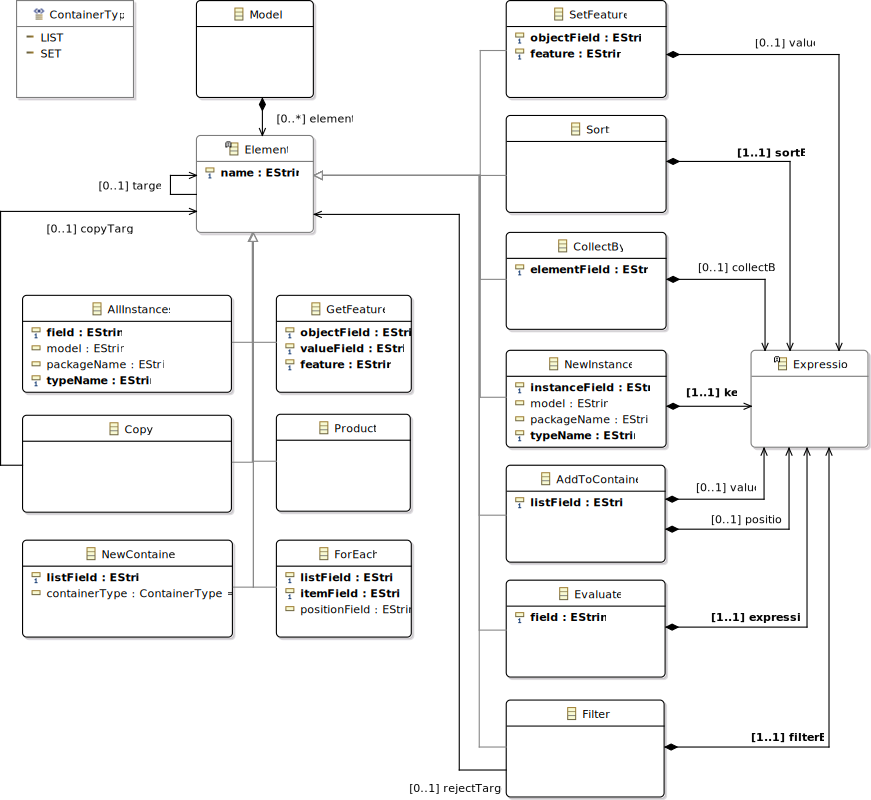
\includegraphics[width=\textwidth]{../dsl/eu.ttc.dataflow.model/model/primitives}
  \caption{Abstract syntax: primitives}
  \label{fig:ast-primitives}
\end{figure}

\begin{figure}
  \centering
  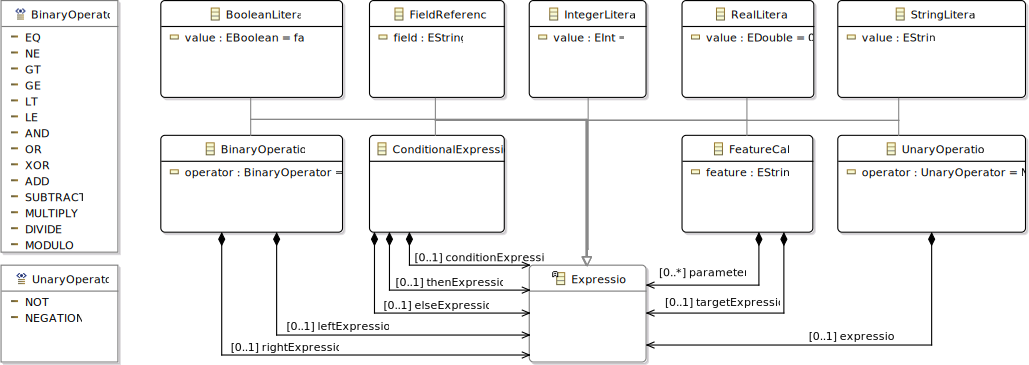
\includegraphics[width=\textwidth]{../dsl/eu.ttc.dataflow.model/model/expressions}  
  \caption{Abstract syntax: expressions}
  \label{fig:ast-expressions}
\end{figure}

\subsubsection{Primitives}

As shown in Figure~\ref{fig:ast-primitives}, a transformation is
defined as a \class{Model} that contains a collection of connected
\class{Element}s. These generally take a sequence of ``rows'' (a
collection of key/value pairings) and process them in some way,
forwarding the resulting tuples to the \emph{target}
\class{Element}. Some elements have more than one possible target in
order to allow for more advanced behaviour (e.g. \class{Filter} can
split tuples into two streams according to a condition).

% AGD: hide primitives which don't need to be implemented?

The primitives can be divided into several groups. First, there are
the object handling primitives:

\begin{itemize}
\item \class{AllInstances}: for each input row $r$, it produces one
  new row $r'$ for each instance of the specified type within the
  specified package and model, where the specified field will be set
  to that instance. Package and model are optional.

  If this step has no incoming edges, it will act as it received a
  single empty row, producing one row per instance of the specified
  type from scratch. It will be very commonly the first step in most
  transformations.

\item \class{NewInstance}: evaluates the \emph{key} expression against
  each input tuple and tests if an instance of the same type was
  previously created against the same key (potentially from another
  \class{NewInstance} step). If it was not, it will set the field
  mentioned in \emph{instanceField} to a new instance of the specified
  type and package within the specified model. Otherwise, it will set
  the same field to the previously created element.

  The usage of a key is meant to provide a similar facility to the
  \emph{equivalent()} operation in popular languages such as ATL or
  ETL.

\item \class{GetFeature}: reads a feature (e.g. an attribute or
  reference) from an object in a field of the input row and places it
  as a field of the output row. Useful in combination with
  \class{AddToContainer} later.

\item \class{SetFeature}: sets a feature of an object to the result of
  a certain \class{Expression} on each input row.
\end{itemize}

There are primitives for computing derived values and operating on
collections:

\begin{itemize}
\item \class{Evaluate}: computes an arbitrary expression on the
  current input row and places it as a field on the output row.

\item \class{NewContainer}: creates a new, empty container as a field
  on each input row. The container may be a set, or a list.

\item \class{AddToContainer}: adds an element (potentially at a
  certain position) to the container present in a certain field of the
  input row. This operation has been treated as a primitive, as it may
  need specific considerations for incremental processing.
\end{itemize}

More primitives are available for managing rows:

\begin{itemize}
\item \class{Filter}: for each input row, evaluates the
  \emph{filterBy} expression. Rows that produce a \emph{true} value
  are sent through the \emph{target} element, and those that produce a
  \emph{false} value are sent through the \emph{rejectTarget} element.

\item \class{Copy}: duplicates the same input rows in the same order
  to the \emph{target} and \emph{copyTarget} elements.

\item \class{Product}: this step is intended to receive rows from two
  \class{Element}s and generate the cartesian product of the two sets
  of rows (e.g. produce all pairs of rows from both elements).

\item \class{Sort}: reads in all the rows and then sorts them
  according to the values produced by the \emph{sortBy} expression.

\item \class{ForEach}: for each input row with a collection on a
  certain field, it produces as many rows as elements in that
  collection, setting a certain field to each of its elements.

\item \class{CollectBy}: for each sequence of contiguous rows with the
  same value for \emph{collectBy}, it will produce one row replacing
  all fields with collections of their respective values in the
  sequence.
\end{itemize}

While these are quite a few primitives, only some of them need to be
implemented to run the transformations proposed in this case
study. The required primitives will be mentioned later on.

\subsubsection{Expressions}

As mentioned above, some of these \class{Element}s can embed
\class{Expression}s in order to compute derived values,
sorting/grouping keys or filtering
conditions. Figure~\ref{fig:ast-expressions} shows the available
elements for the small expression language. The objective of the
language is to be side-effect free as much as possible. An expression
is a tree of elements of various types:

\begin{itemize}
\item Literals of a certain type, e.g. \class{BooleanLiteral} for
  boolean values and so forth.

\item \class{FieldReference}s to a certain field within the row, by
  name.

\item \class{UnaryOperation}s, which take the result of a
  subexpression and apply to it logical negation (\emph{NOT} in
  \class{UnaryOperator}) or arithmetic negation (\emph{NEGATION}).

\item \class{BinaryOperation}s, which combine the result of two
  subexpressions in various ways. The language supports equality
  comparison (\emph{EQ} in \class{BinaryOperator}), inequality
  (\emph{NE}), greater than (\emph{GT}), greater or equal (\emph{GE}),
  less than (\emph{LT}), less or equal (\emph{LE}), logical AND with
  shortcircuit, logical OR with shortcircuit, logical XOR, numeric
  addition / string concatenation (\emph{ADD}), subtraction,
  multiplication, division or the modulo operation.

  \emph{Note}: to simplify some cases, logical operators operate with
  ``truish'' values as well (as in JavaScript). A ``truish'' value is
  a ``true'' Boolean literal, a non-empty string, a non-null EObject,
  a non-empty sequence or a non-zero number.

\item \class{FeatureCall}s, which access a certain property or method
  within an object contained in the present row. If it is a method
  call, it will include a list of parameter subexpressions. The
  transformations to be run assume that ``a.x'' will be translated to
  ``a.eGet(feature x)'' in EMF terms, and that ``a.eClass'' and
  ``a.eContainer'' will also be available.

\item \class{ConditionalExpression}s, inspired by the ternary operator
  in C/C++ and by the \emph{if..then..else} expression in Python. If
  the conditional expression produces a \emph{true} value it will
  compute and return the result of the \emph{thenExpression},
  otherwise it will use the \emph{elseExpression}.
\end{itemize}

\subsection{Example: Families to Persons}
\label{sec:f2p}

Since the current case study does not involve writing new
transformations but rather executing existing ones, the concrete
syntax will be simply illustrated through the basic example to be
executed: the classic ``Families to Persons'' transformation, as
listed in the ATL
Zoo\footnote{\url{https://www.eclipse.org/atl/atlTransformations/#Families2Persons}}.

This transformation takes a collection of \class{Family} instances
containing \class{Member}s, whose genders are derived from their role
in the \class{Family}, and transforms them into either \class{Male} or
\class{Female} instances depending on their gender, while preserving
their first and last names.

Two concrete syntaxes are provided in the Github repository for the
abstract syntax shown in Section~\ref{sec:asyn}. The main syntax is
textual (Xtext-based) and similar to OMG HUTN~\cite{hutn2004},
allowing users to comfortably write the embedded expressions included
in primitives such as \class{Evaluate} or \class{Filter}. A graphical
syntax has also been developed using Sirius, for simpler visualization
of the connections between the primitives. The same model can be
edited through both notations at the same time, thanks to the
viewpoint approach taken by Sirius.

\lstinputlisting[float,label=lst:f2p,caption={Families to Persons, textual \FlowMM notation},language=FlowM2M,numbers=left,numberstyle=\scriptsize,frame=tb,columns=flexible,basicstyle=\small]{../examples/eu.ttc.dataflow.examples.families2persons/transformation/families2persons.dataflow}

The textual representation of the ``Families to Persons'' example is
shown in Listing~\ref{lst:f2p}. The transformation starts by
retrieving all the instances of \class{Member} in ``AllMembers'', and
then computing the full name in advance through the
``ComputeFullName'' element. ``SplitByGender'' receives the resulting
rows and distributes them between the ``NewMale'' and ``NewFemale''
elements. This creates the appropriate \class{Male} or \class{Female}
instance, which is sent to ``SetPersonName'' to have its full name
set.

\begin{figure}
  \centering
  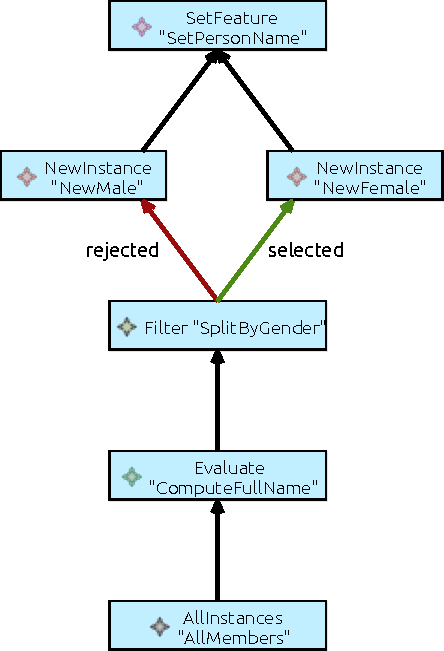
\includegraphics[width=.4\textwidth]{families2persons}
  \caption{Families to Persons, graphical \FlowMM notation}
  \label{fig:f2p}
\end{figure}

The graphical representation of the ``Families to Persons'' example is
shown in Figure~\ref{fig:f2p}. As it can be seen, it is only meant to
be a viewpoint on the full model that emphasizes the flows between the
different activities: it does not represent the embedded expressions
themselves. The representation is mostly a simple ``boxes and arrows''
affair, mentioning the primitive type and the name of the
\class{Element}. This partial representation is editable,
nevertheless, as it can be useful for detecting disconnected or
wrongly connected elements in the flow. For clarity, the outgoing
edges of the \class{Filter} steps are color-coded and labelled
depending on whether they take the rows that passed the condition or
not.

\subsection{Task 1: base primitives}
\label{sec:baseprim}

% tree2graph: AllInstances, Evaluate, Filter, NewInstance, SetFeature
% families2persons: AllInstances, Evaluate, Filter, NewInstance, SetFeature

The first task of this case study is implementing an approach that
enables the batch and/or incremental execution of two basic
transformations: the ``Families to Persons'' example shown in
Section~\ref{sec:f2p} and a ``Tree to Graph'' transformation that was
also inspired from a case in the ATL Transformation Zoo. Both
transformations are available as subfolders of the \file{examples}
folder in the GitHub repository.

The basic folder layout is the same for all examples:
\begin{itemize}
\item \file{input}: manually constructed model, plus a set of small,
  medium and large synthetic models (with the \file{GS}, \file{GM} and
  \file{GL} suffixes, respectively).
\item \file{output}: expected output for the manually constructed
  example.
\item \file{metamodels}: Ecore metamodels for the input and output
  models.
\item \file{generator}: the Epsilon Model
  Generator\footnote{\url{https://github.com/sop501/ModelCodes}}
  script that produced the synthetic models.
\item \file{transformation}: a \file{.dataflow} file specifying the
  transformation according to the abstract syntax in
  Section~\ref{sec:asyn} and the textual concrete syntax used in
  Listing~\ref{lst:f2p}.
\item The root folder of the example contains a \file{.launchconfig}
  with the Ecore-based launch configuration used for the sample
  Epsilon-based interpreter, a set of Eclipse launch configurations to
  use the model generator, and an \file{.aird} file with a graphical
  representation of the transformation.
\end{itemize}

A reference Epsilon\footnote{\url{http://eclipse.org/epsilon}}-based
interpreter of \file{.dataflow} files is available in
\file{solutions}. It is not designed for performance nor scalability,
however: contestants are free to use their favorite approach to enable
execution (e.g. Java code generation, transformation to another tool
or better interpretation). Contestants are also invited to slightly
tweak semantics if it improves incrementality, maintainability or
performance, as long as the transformation produces the intended
result.

The base set of primitives for this task are \class{AllInstances},
\class{Evaluate}, \class{Filter}, \class{NewInstance} and
\class{SetFeature}. Contestants are free to limit the implementation
of the expression language to the particular operators and methods
that are required by these transformations.

% tree2graph: AllInstances, Evaluate, Filter, NewInstance, SetFeature
% families2persons: AllInstances, Evaluate, Filter, NewInstance, SetFeature

\subsection{Task 2: extended primitives}
\label{sec:extprim}

% flowchart2html: base + ForEach, AddToContainer
% flowchart2html-alt: flowchart2html + conditional expressions
% class2rdb: base + AddToContainer

The second task is a direct extension of the first one: this time, the
two transformations to be enabled are more complex. One is an instance
of the (in)famous ``Class to RDB'' example, while the other is a
``Flowchart to HTML'' transformation. These transformations follow the
same folder layout mentioned in Section~\ref{sec:baseprim}.

This task requires implementing the primitives in the previous task,
plus the \class{ForEach} and \class{AddToContainer} tasks. The fact
that these primitives handle collections will naturally complicate
their execution, especially in an incremental scenario. As for the
expression language, more operators will have to be implemented: in
particular, ``Flowchart to HTML'' includes an alternative version that
takes advantage of the ternary ``if...then...else...'' operator.

\section{Evaluation}
\label{sec:eval}

Contestants should submit their solutions at the end of the day before
the contest in a form that allows for easy execution by
attendees. Solutions will be submitted as pull requests to the main
GitHub repository, adding new subfolders to the \file{solutions}
folder. Solutions should also report their execution times in
milliseconds, to aid performance evaluation.

The solutions shall be evaluated according to the following criteria:
\begin{itemize}
\item Batch correctness -- how many of the manually constructed models
  are transformed correctly?

\item Incremental correctness -- how many of the manually constructed
  models are recalculated/updated correctly after a change in the
  model?

  The actual changes to the model will be:
  \begin{itemize}
  \item For ``Families to Persons'': change the role of a member of a
    family, so that their gender changes.
  \item For ``Tree to Graph'': remove a subtree, which should result
    in removing a subgraph.
  \item For ``Class to RDB'': add a new multivalued scalar attribute,
    producing a new table.
  \item For ``Flowchart to HTML'': add a new transition, which should
    result in a new link.
  \end{itemize}

\item Batch performance -- is the solution faster than the others at
  transforming the large synthetic model? \emph{Requires batch
    correctness.}

\item Incremental performance -- is the solution faster than the
  others at producing the updated model after changing the large
  synthetic model as mentioned above? \emph{Requires incremental
  correctness.}

\item Maintainability and extensibility -- can the provided solution
  be extended naturally to cover the other primitives which were not
  used in this case study?
\end{itemize}

\bibliographystyle{plain}
\bibliography{bibliography}

\end{document}
